\documentclass[12pt]{article}
\usepackage{titlesec}
\usepackage{subcaption}
\usepackage[scaled]{helvet}  \renewcommand\familydefault{\sfdefault} % Font
\usepackage{graphicx} % Required for inserting images
\usepackage{geometry}
\usepackage{pgfplotstable}
\usepackage{amsmath}
\usepackage{enumitem}
\usepackage{tikz} 
\usetikzlibrary{petri,arrows.meta}
\geometry{a4paper, total={170mm,257mm},left=20mm, top=20mm,}
\usepackage[listings,breakable,skins]{tcolorbox}
% declare our code block environment
  \newtcblisting{tcbcodeblock}[1]{%
    enhanced,
    sharp corners,
    colframe=black,
    coltext=codefg,
    colback=codebg,
    breakable,
    size=fbox,
    listing only,
    listing options={%
      style=tcblatex,
      language={#1},
      showspaces=false,
      showstringspaces=false,
      commentstyle=\color{codegray},
      keywordstyle=\color{codegreen},
      stringstyle=\color{codecyan},
      basicstyle=\ttfamily\footnotesize
    }
  }
\renewcommand{\thesection}{\Roman{section}}
\renewcommand{\thesubsection}{\arabic{subsection}}
\renewcommand{\thesubsubsection}{\alph{subsubsection}.}

\titleformat{\section}{\normalfont\LARGE\bfseries}{\thesection.}{10pt}{}
\titleformat{\subsection}{\normalfont\Large}{\thesubsection.}{10pt}{}
\titleformat{\subsubsection}{\normalfont\large}{\thesubsubsection}{10pt}{}

\begin{document}
\thispagestyle{empty} %Suppress number of this page
\begin{center}
    \vspace{7pt}
    \fontsize{18pt}{17pt}\selectfont 
    \textbf{University of Science and Technology of Hanoi}
    \vspace{7pt}
\end{center}
\vspace{10pt}
\begin{center}
    
\includegraphics[scale=0.4]{USTH.png}
\end{center}

\vspace{90pt}

\begin{center}
    \fontsize{30pt}{17pt}\selectfont 
    \textbf{Deep learning} 
    \vspace{50pt}

    \fontsize{20pt}{17pt}\selectfont 
    \textbf{Report 2 Linear regression}
    \vspace{50pt}


    \fontsize{17pt}{17pt}\selectfont
    \textbf{{Student id: }{ict2440050}}
    \vspace{15pt}

    \fontsize{17pt}{17pt}\selectfont
    \textbf{{Student name: }{Nguyen Vu Bach}}
    \vspace{15pt}
    
\end{center}

\newpage
\setcounter{page}{1} % Start number from this page
\section{How did I implement the algorithm}

\subsection{Initialize learning rate and weights}

\subsection{Iteratively updates \( w_1 \) and \( w_0 \)}
\begin{itemize}
    \item Apply gradient descend on \( w_1 \) and \( w_0 \)
    \begin{equation}
    \frac{\partial L}{\partial w_0} = \sum_{i=1}^n (\hat{y}_i - y_i) = \sum_{i=1}^n (w_1 x_i + w_0 - y_i)
\end{equation}

\begin{equation}
    \frac{\partial L}{\partial w_1} = \sum_{i=1}^n x_i (\hat{y}_i - y_i) = \sum_{i=1}^n x_i (w_1 x_i + w_0 - y_i)
\end{equation}

    \item Update \( w_1 \) and \( w_0 \) using learning rate:
\begin{equation}
    w_0 = w_0 - lr \cdot \frac{\partial L}{\partial w_0}, \quad w_1 = w_1 - lr \cdot \frac{\partial L}{\partial w_1}
\end{equation}

    \item Repeat gradient descend then update

\end{itemize}

\subsection{Compute Loss function}

\begin{equation}
    L(w_1, w_0) = \frac{1}{2} \sum_{i=1}^n (w_1 x_i + w_0 - y_i)^2
\end{equation}

Where
\begin{itemize}
    \item \( w_1 \) and \( w_0 \) are current weights
    \item \(x_i\) and \(y_i\) are the provided data
\end{itemize}

\newpage

\section{Analyze the effect of different learning rate for convergence}
\begin{itemize}
    \item For lr = 0.0001
        \begin{figure}[h!]
            \centering
            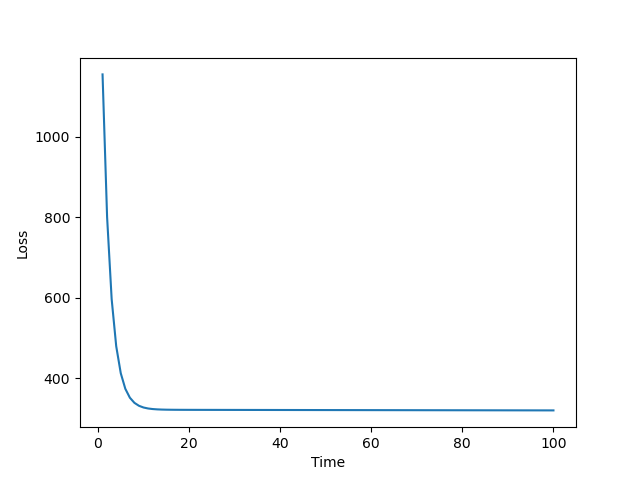
\includegraphics[width=0.7\linewidth]{images/Lab2/Good.png}
            \caption{Loss function of learning rate 0.0001}
        \end{figure}

    \item For lr = 0.00001
        \begin{figure}[h!]
            \centering
            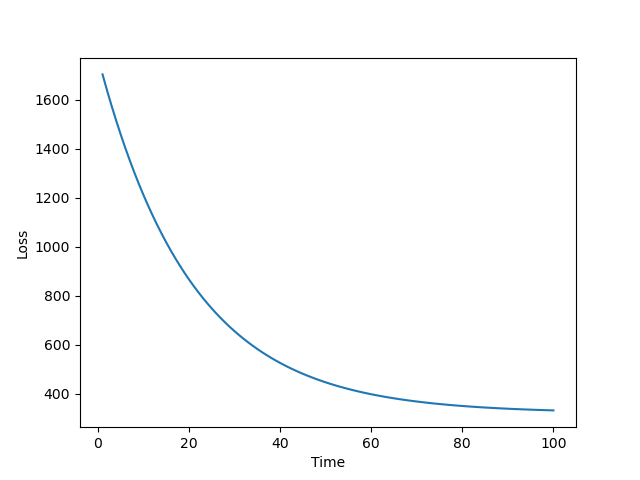
\includegraphics[width=0.7\linewidth]{images/Lab2/Small.png}
            \caption{Loss function of learning rate 0.00001}
        \end{figure}
        
\newpage
    \item For lr = 0.001
        \begin{figure}[h!]
            \centering
            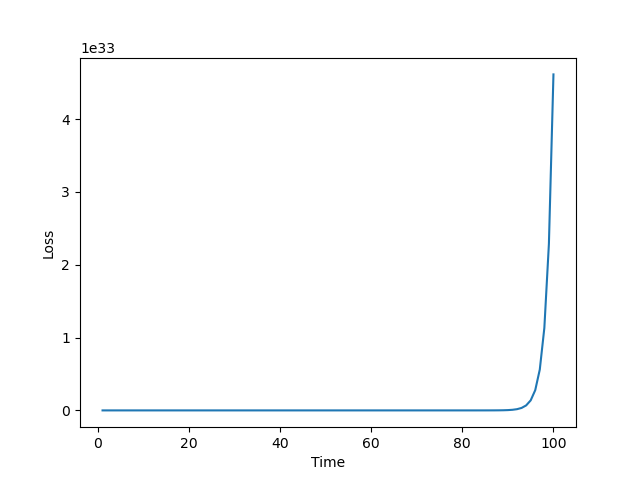
\includegraphics[width=0.7\linewidth]{images/Lab2/Big.png}
            \caption{Loss function of learning rate 0.001}
        \end{figure}

    \item Conclusion: Excessively high learning rates may cause divergence or oscillations, while overly low rates can lead to slow convergence or getting stuck in local minima.

\end{itemize}


% \begin{table}[h!]
%     \centering
%     \begin{tabular}{c c c} \hline
%     Format & Min & Max  \\ \hline
%     32-bit floating-point & -1 & +1 \\
%     32-bit integer PCM & \(-2^{31}\) & \(+2^{31}\)\\
%     24-bit integer PCM & \(-2^{23}\) & \(+2^{23}\)\\
%     16-bit integer PCM & \(-2^{15}\) & \(+2^{15}\) \\
%     8-bit integer PCM & 0 & 255 \\ \hline
%     \end{tabular}
%     \caption{Some common data type}
%     \label{sec1:dtype}
% \end{table}


\end{document}







